
\section{Analisi dei Requisiti} \label{sec:analisi}
\subsection{Casi d'uso} \label{sec:casiduso}
In questa sezione verranno elencati i casi d'uso del sistema che è oggetto dello stage. Dato che il sistema è stato pensato per rispondere solo all'intervento di un utente che si occupa di amministrazione e installazione l'unico attore che prenderemo in considerazione è \textbf{utente}. Per ogni caso d'uso verranno riportate:
\begin{enumerate}
\item DESCRIZIONE: contenuto del caso d'uso
\item FLUSSO PRINCIPALE DEGLI EVENTI
\item PRECONDIZIONI: asserzioni che sono valide prima dell'effettiva esecuzione del caso d'uso
\item POSTCONDIZIONI: asserzioni che sono valide dopo l'esecuzione del caso d'uso
\item SCENARI ALTERNATIVI: eventuali scenari alternativi che differiscono dal normale flusso del caso d'uso
\end{enumerate}
Ogni caso d'uso ha un identificativo stile UC\textit{n} dove n indica una posizione gerarchica.
Ogni caso d'uso è posizionato all'interno della gerarchia che parte dal caso d'uso più generale UC0 (radice dell'albero). Per ogni caso d'uso figlio valgono le precondizioni del padre.

\subsection{UC0: Scenario Principale} \label{sec:uc0}
\begin{description}
 \item[\em{descrizione}] L'utente ha avviato il sistema il quale è pronto a rispondere agli eventi. L'utente può scegliere di accedere alla calibrazione delle telecamere, accedere alla loro configurazione, oppure generare le statistiche a partire dai dati di tracking attualmente presenti nel sistema (figura ~\ref{fig:uc0})
 
\item[\em{flusso principale degli eventi}] \mbox{}
 \begin{enumerate}
	\item L'utente può calibrare le telecamere (\hyperref[sec:uc1]{UC1}) 
	\item L'utente può configurare le telecamere (\hyperref[sec:uc2]{UC2})
	\item L'utente può generare e visualizzare le statistiche (\hyperref[sec:uc3]{UC3})
\end{enumerate} 
 \item[\em{precondizione}] Il sistema è avviato e funzionante \end{description}
\begin{figure}[htpb]
\centering
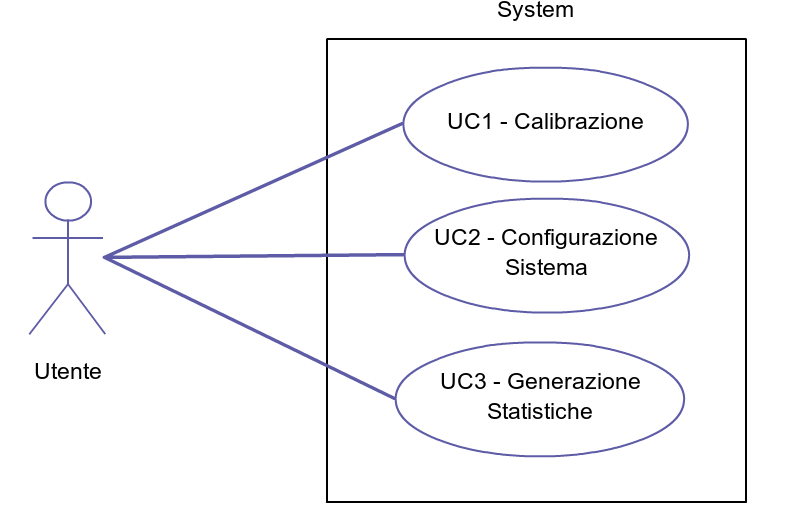
\includegraphics[scale=0.4]{./images/uc0.png}
\caption{UC0 - Scenario principale}
\label{fig:uc0}
\end{figure} 
 

\subsection{UC1: Calibrazione telecamere} \label{sec:uc1}
\begin{description}
 \item[\em{descrizione}] L'utente può iniziare la calibrazione delle telecamere, oppure può visualizzare un video \textit{undistorted} che usa i parametri di calibrazione per correggere i frame prodotti dal video. (figura ~\ref{fig:uc1})
 \item[\em{flusso principale degli eventi}] \mbox{}
 \begin{enumerate}
	\item L'utente può iniziare la calibrazione (\hyperref[sec:uc1.1]{UC1.1}) 
	\item L'utente può visualizzare il video corretto con i parametri di calibrazione (\hyperref[sec:uc1.2]{UC1.2})
\end{enumerate} 
 \item[\em{precondizione}] Il sistema è avviato e funzionante

\end{description}
 
\begin{figure}[htpb]
\centering
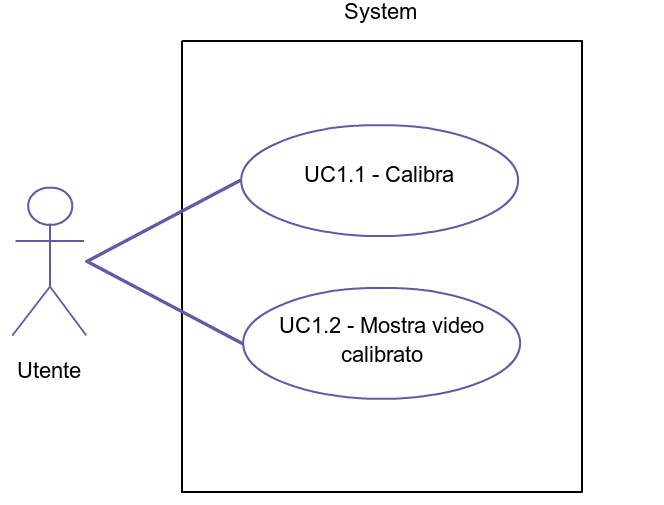
\includegraphics[scale=0.4]{./images/uc1.png}
\caption{UC1 - Calibrazione telecamere}
\label{fig:uc1}
\end{figure} 

\subsubsection{UC1.1: Calibra} \label{sec:uc1.1}
\begin{description}
 \item[\em{descrizione}] L'utente sta selezionando le opzioni per la calibrazione delle telecamere. Può selezionare: numero di span spot della scacchiera, numero di frame da scartare durante la calibrazione, indirizzo IP nella rete della camera da calibrare, e poi iniziare l'effettiva calibrazione.  (figura ~\ref{fig:uc1.1})
 
 \item[\em{flusso principale degli eventi}] \mbox{}
 \begin{enumerate}
	\item L'utente seleziona il numero di span spot (\hyperref[sec:uc1.1.1]{UC1.1.1})
	\item L'utente seleziona il numero frame da scartare (\hyperref[sec:uc1.1.2]{UC1.1.2})
	\item L'utente seleziona l'indirizzo della camera da calibrare (\hyperref[sec:uc1.1.3]{UC1.1.3})
	\item L'utente avvia la calibrazione calibrare (\hyperref[sec:uc1.1.4]{UC1.1.4})
\end{enumerate}  
  \item[\em{postcondizione}] I file che contengono i file di
  calibrazione della telecamera (extrinsics e instrinsics) sono stati generati e salvati nel file system
  \item[\em{scenari alternativi}] \mbox{}
  \begin{enumerate}
	\item L'utente interrompe la procedura, il sistema torna in attesa di eventi
	\item La procedura di calibrazione fallisce, il sistema segnala l'errore e torna in attesa di eventi
\end{enumerate} 
 \end{description}
\begin{figure}[htpb]
\centering
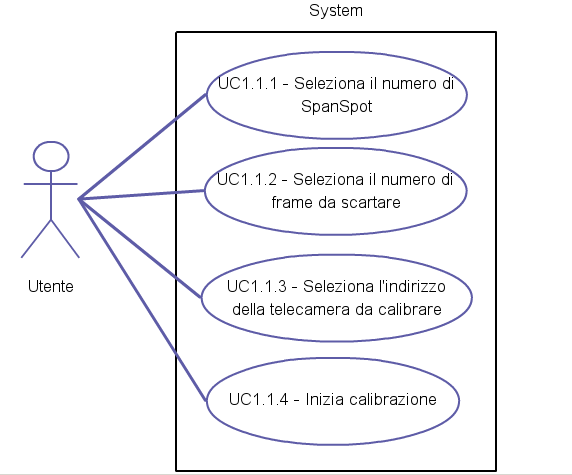
\includegraphics[scale=0.4]{./images/uc11.png}
\caption{UC1.1 - Calibra}
\label{fig:uc1.1}
\end{figure} 

\paragraph{UC1.1.1: Seleziona il numero di span spot} \label{sec:uc1.1.1}
\begin{description}
 \item[\em{descrizione}] L'utente seleziona il numero di span spot per la calibrazione
 \item[\em{postcondizione}] Il sistema conosce il numero di span spot da utilizzare nella calibrazione
  \item[\em{scenari alternativi}] \mbox{}
  \begin{enumerate} 
  \item L'utente interrompe la procedura, il sistema ritorna in attesa di eventi
  \end{enumerate}
 \end{description}

\paragraph{UC1.1.2: Seleziona il numero di frame da scartare} \label{sec:uc1.1.2}
\begin{description}
 \item[\em{descrizione}] L'utente seleziona il numero di frame da scartare per la calibrazione
 \item[\em{precondizione}] L'utente ha già selezionato il numero di span spot
 \item[\em{postcondizione}] Il sistema conosce il numero di frame da scartare nella calibrazione
 \item[\em{scenari alternativi}] \mbox{}
  \begin{enumerate}
  \item L'utente interrompe la procedura, il sistema ritorna in attesa di eventi
  \end{enumerate}
 \end{description}

\paragraph{UC1.1.3: Inserisce l'indirizzo della telecamera da calibrare} \label{sec:uc1.1.3}
\begin{description}
 \item[\em{descrizione}] L'utente inserisce l'indirizzo della telecamera da calibrare
 \item[\em{precondizione}] L'utente ha già selezionato il numero di span spot e il numero di frame da scartare nella calibrazione
 \item[\em{postcondizione}] Il sistema conosce l'indirizzo della telecamera da calibrare
  \item[\em{scenari alternativi}]  \mbox{}  \begin{enumerate}
  \item L'utente interrompe la procedura, il sistema ritorna in attesa di eventi
  \end{enumerate}
 \end{description}

\paragraph{UC1.1.4: Inizia calibrazione} \label{sec:uc1.1.4}
\begin{description}
 \item[\em{descrizione}] L'utente inizia la calibrazione effettiva
 \item[\em{precondizione}] L'utente ha già selezionato le opzioni di calibrazione (UC1.1.1 - UC1.1.2 - UC1.1.3), il sistema quindi conosce i parametri da utilizzare
 \item[\em{postcondizione}] Il sistema genera i file di calibrazione intrinsics ed extrinsics e li salva nel file system
   \item[\em{scenari alternativi}]  \mbox{}
    \begin{enumerate} 
  \item La calibrazione non termina con successo quindi l'operazione viene interrotta e l'errore segnalato. Il sistema ritorna in attesa di eventi
  \end{enumerate}
 \end{description}

\subsection{UC1.2: Mostra video calibrato} \label{sec:uc1.2}
\begin{description}
 \item[\em{descrizione}] L'utente visualizza il video corretto con i valori di calibrazione
 \item[\em{precondizione}] L'utente ha già effettuato con successo la generazione dei file di calibrazione che sono presenti nel sistema
 
\end{description}


\subsection{UC2: Configurazione telecamere} \label{sec:uc2}
\begin{description}
 \item[\em{descrizione}] L'utente può impostare le opzioni di configurazione delle telecamere, aggiungendone di nuove, rimuovendole, modificandole. Può inoltre ottenere i file necessari alla configurazione, convertendo un file .DXF in .PNG, salvando un frame dalla telecamera, o calcolare la \textit{homography matrix} (figura ~\ref{fig:uc2})
 
\item[\em{flusso principale degli eventi}] \mbox{}
 \begin{enumerate}
	\item L'utente inserisce una nuova telecamera nel sistema (\hyperref[sec:uc2.1]{UC2.1})
	\item L'utente rimuove una telecamera esistente (\hyperref[sec:uc2.2]{UC2.2})
	\item L'utente modifica la configurazione di una telecamera (\hyperref[sec:uc2.3]{UC2.3})
	\item L'utente cattura e salva un frame della telecamera (\hyperref[sec:uc2.4]{UC2.4})
		\item L'utente converte un file .DXF in .PNG (\hyperref[sec:uc2.5]{UC2.5})
			\item L'utente calcola la matrice omografica relativa ad una telecamera (\hyperref[sec:uc2.6]{UC2.6})
		\item L'utente seleziona una telecamera (\hyperref[sec:uc2.7]{UC2.7})
\end{enumerate}
 \item[\em{precondizione}] Il sistema è avviato e funzionante. \end{description}
\begin{figure}[htpb]
\centering
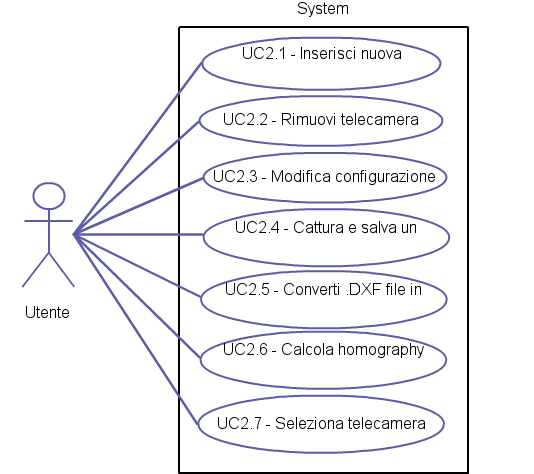
\includegraphics[scale=0.4]{./images/uc2.png}
\caption{UC2 - Configurazione telecamere}
\label{fig:uc2}
\end{figure} 

\subsubsection{UC2.1: Inserisci nuova} \label{sec:uc2.1}
\begin{description}
 \item[\em{descrizione}] L'utente inserisce il nome della nuova telecamera
 \item[\em{postcondizione}] Il sistema ha inserito la nuova telecamera nel database
\item[\em{scenari alternativi}]  \mbox{}
    \begin{enumerate} 
  \item Il nome inserito non è valido, il sistema interrompe l'operazione e torna in attesa di eventi.
  \end{enumerate} 
 \end{description}

\subsubsection{UC2.2: Rimuovi telecamera}\label{sec:uc2.2}
\begin{description}
 \item[\em{descrizione}] L'utente rimuove la telecamera selezionata
  \item[\em{precondizione}] L'utente ha selezionato una telecamera tra quelle esistenti
 \item[\em{postcondizione}] Il sistema ha rimosso la telecamera dal database
 \end{description}
 
\subsubsection{UC2.3: Modifica configurazione} \label{sec:uc2.3}
\begin{description}
 \item[\em{descrizione}] L'utente ha selezionato una telecamera e ne modifica le opzioni di configurazione, quali: file extrinsics, intrinsics, valore dell'altezza del frame, valore della larghezza del frame, percorso del file contentente la \textit{homography matrix} (figura ~\ref{fig:uc23}).
 
\item[\em{flusso principale degli eventi}] \mbox{}
 \begin{enumerate}
	\item L'utente modifica il percorso del file di calibrazione \textit{extrinsics} (\hyperref[sec:uc2.3.1]{UC2.3.1})
	\item L'utente r modifica il percorso del file di calibrazione \textit{intrinsics} (\hyperref[sec:uc2.3.2]{UC2.3.2})
	\item L'utente modifica il valore dell'altezza del frame (\hyperref[sec:uc2.3.3]{UC2.3.3})
	\item L'utente modifica il valore della larghezza del frame (\hyperref[sec:uc2.3.4]{UC2.3.4})
		\item L'utente modifica il percorso del file di configurazione contenente la \textit{homography matrix} (\hyperref[sec:uc2.3.5]{UC2.3.5})
\end{enumerate}    
 
  \item[\em{precondizione}] L'utente ha selezionato una telecamera tra quelle esistenti
  
\item[\em{scenari alternativi}]  \mbox{}
    \begin{enumerate} 
  \item L'utente interrompe la modifica, il sistema ritorna in attesa di eventi
  \end{enumerate}   
 \end{description}
 \begin{figure}[htpb]
\centering
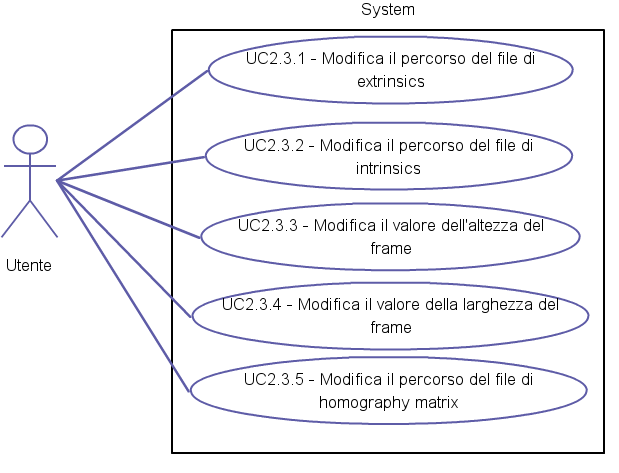
\includegraphics[scale=0.4]{./images/uc23.png}
\caption{UC2.3 - Modifica telecamere}
\label{fig:uc23}
\end{figure} 

\paragraph{UC2.3.1: Modifica il percorso del file di extrinsics} \label{sec:uc2.3.1}
\begin{description}
 \item[\em{descrizione}] L'utente seleziona un file nel file system che contiene i valori \textit{extrinsics} di calibrazione.
   \item[\em{postcondizione}] Il sistema ha modificato il corrispondente valore della telecamera nel database
  \item[\em{scenari alternativi}] \mbox{}
  \begin{enumerate}
  \item L'utente interrompe la selezione del file, il sistema ritorna in attesa di eventi
  \end{enumerate}
 \end{description}

\paragraph{UC2.3.2: Modifica il percorso del file di intrinsics} \label{sec:uc2.3.2}
\begin{description}
 \item[\em{descrizione}] L'utente seleziona un file nel file system che contiene i valori \textit{intrinsics} di calibrazione.
   \item[\em{postcondizione}] Il sistema ha modificato il corrispondente valore della telecamera nel database
     \item[\em{scenari alternativi}] \mbox{}
  \begin{enumerate}
  \item L'utente interrompe la selezione del file, il sistema ritorna in attesa di eventi
  \end{enumerate}
 \end{description}

\paragraph{UC2.3.3: Modifica il valore dell'altezza del frame}
\begin{description}  \label{sec:uc2.3.3}
 \item[\em{descrizione}] L'utente seleziona un valore per l'altezza del frame della telecamera.
   \item[\em{postcondizione}] Il sistema ha modificato il corrispondente valore della telecamera nel database
 \end{description}
 
\paragraph{UC2.3.4: Modifica il valore della larghezza del frame}  \label{sec:uc2.3.4}
\begin{description}
 \item[\em{descrizione}] L'utente seleziona un valore per la larghezza del frame della telecamera.
   \item[\em{postcondizione}] Il sistema ha modificato il corrispondente valore della telecamera nel database
 \end{description}
 
 \paragraph{UC2.3.5: Modifica il percorso del file di homography matrix} \label{sec:uc2.3.5}
\begin{description}
 \item[\em{descrizione}] L'utente seleziona un file nel file system che contiene i valori che descrivono la  \textit{homography matrix} utilizzata per la traduzione delle coordinate.
   \item[\em{postcondizione}] Il sistema ha modificato il corrispondente valore della telecamera nel database
   \item[\em{scenari alternativi}] \mbox{}
  \begin{enumerate}
  \item L'utente interrompe la selezione del file, il sistema ritorna in attesa di eventi
  \end{enumerate}
 \end{description}
 
 
\subsubsection{UC2.4: Cattura e salva un frame della telecamera} \label{sec:uc2.4}
 \begin{description}
 \item[\em{descrizione}] L'utente indica al sistema di attivare la telecamera selezionata, catturare un frame e salvarlo.
  
  \item[\em{precondizione}] L'utente ha selezionato una telecamera tra quelle esistenti
  
  \item[\em{postcondizione}] Il frame della telecamera selezionata è stato salvato nel file system
  
\item[\em{scenari alternativi}]  \mbox{}
    \begin{enumerate} 
  \item La telecamera non è raggiungibile, il sistema interrompe l'operazione segnala l'errore e ritorna in attesa di eventi
  \end{enumerate}   
 \end{description}
 
 \subsubsection{UC2.5: Converti .DXF file in .PNG} \label{sec:uc2.5}
 \begin{description}
 \item[\em{descrizione}] L'utente seleziona nel file system un file .DXF da convertire in formato .PNG 
    
  \item[\em{postcondizione}] Il file selezionato è stato convertito in un immagine che riproduce il contenuto del .DXF
  
 \end{description}
 
 \subsubsection{UC2.6: Calcola homography matrix} \label{sec:uc2.6}
 \begin{description}
 \item[\em{descrizione}] L'utente calcola la homography matrix per una particolare telecamera configurata.
  \item[\em{postcondizione}] Il file che contiene la \textit{homography matrix} è stato calcolato e salvato nel file system
  
 \end{description}
 
  \subsubsection{UC2.7: Seleziona telecamera} \label{sec:uc2.7}
 \begin{description}
 \item[\em{descrizione}] L'utente seleziona una telecamera tra la lista di telecamere presenti nel sistema
  \item[\em{postcondizione}] La telecamera indicata diventa selezionata e quindi \textbf{attiva}
  
 \end{description}
 
 
 
\subsection{UC3: Generazione statistiche} \label{sec:uc3}
\begin{description}
 \item[\em{descrizione}] L'utente può visualizzare le statistiche relative ai dati presenti nel sistema. Può effettuare la conversione dei dati \textit{raw}, visualizzare l'\textit{heatmap}, o le statistiche (figura ~\ref{fig:uc3})

\item[\em{flusso principale degli eventi}] \mbox{}
 \begin{enumerate}
	\item L'utente seleziona la trasformazione dei dati di tracciamento presenti nel sistema (\hyperref[sec:uc3.1]{UC3.1})
	\item L'utente seleziona la generazione dell'heatmap (\hyperref[sec:uc3.2]{UC3.2})
	\item L'utente seleziona la generazione delle statistiche (\hyperref[sec:uc3.3]{UC3.3})
\end{enumerate}     
 
 \item[\em{precondizione}] Il sistema è avviato e funzionante.
  \end{description}
\begin{figure}[htpb]
\centering
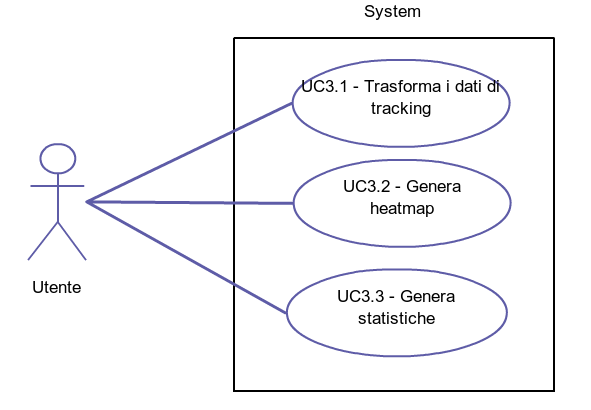
\includegraphics[scale=0.4]{./images/uc3.png}
\caption{UC2 - Generazione statistiche}
\label{fig:uc3}
\end{figure}  
 
\subsubsection{UC3.1: Trasforma i dati di tracking} \label{sec:uc3.1}
\begin{description}
 \item[\em{descrizione}] L'utente indica al sistema di eseguire la trasformazione dei dati \textit{raw} di tracking
  \item[\em{postcondizione}] Il sistema ha trasformato i dati presenti nel database ed ha salvato i dati trasformati.
  
  \item[\em{scenari alternativi}]  \mbox{}
    \begin{enumerate} 
  \item La trasformazione fallisce, il sistema segnala l'errore e torna in attesa di eventi
  \end{enumerate}  
  
  \end{description}
  
\subsubsection{UC3.2: Genera heatmap} \label{sec:uc3.2}
\begin{description}
 \item[\em{descrizione}] L'utente indica al sistema di generare l'heatmap con la rappresentazione grafica dei dati di tracking
  \item[\em{postcondizione}] Il sistema elabora i dati presenti nel database generando l'heatmap e salvandola nel file system.
  
\item[\em{scenari alternativi}] \mbox{}
  \begin{enumerate}
  \item La generazione fallisce, il sistema segnala l'errore e torna nello stato di attesa.
  \end{enumerate}  
  \end{description}
  
  
\subsubsection{UC3.3: Genera statistiche} \label{sec:uc3.3}
\begin{description}
 \item[\em{descrizione}] L'utente indica al sistema di generare le statistiche relative ai dati presenti
  \item[\em{postcondizione}] Il sistema ha generato le statistiche e le ha salvate nel database
  
\item[\em{scenari alternativi}] \mbox{}
  \begin{enumerate}
  \item La generazione fallisce, il sistema segnala l'errore e torna nello stato di attesa.
  \end{enumerate}  
  \end{description}  
  
  
  
\subsection{Requisiti} \label{sec:req}
In questa sezione verranno elencati i requisiti software che sono emersi dai casi d'uso individuati e dalle riunioni informative con i leader dello sviluppo. Per chiarezza si è cercato di tenere un rapporto 1:1 tra casi d'uso e requisiti.
 \\ \\Nell'esposizione si userà la seguente convenzione: se un requisito padre ha figli con tipologia diversa tra di loro, il requisito padre assumerà la tipologia più vincolante tra quelle dei figli (esempio: se ci sono 2 figli, uno obbligatorio ed uno desiderabile il padre sarà qualificato come obbligatorio).
\subsubsection{Requisiti funzionali} \label{sec:reqfun}
\begin{center}
    \begin{longtable}{ | l | p{5cm} | c | p{1.5cm} |}
    \caption{Tabella requisiti funzionali} \\
    \hline 
    \textbf{Codice} & \textbf{Descrizione} & \textbf{Tipologia} & \textbf{Fonte} \\ \hline
\endfirsthead
\multicolumn{4}{c}%
{\tablename\ \thetable\ -- \textit{Continued from previous page}} \\
\hline
\textbf{Codice} & \textbf{Descrizione} & \textbf{Tipologia} & \textbf{Fonte} \\
\hline
\endhead
\hline \multicolumn{4}{r}{\textit{Continued on next page}} \\
\endfoot
\hline
\endlastfoot
    RF1 & Il sistema deve permettere all'utente di eseguire la calibrazione delle telecamere & Obbligatorio & UC1
    \\ \hline
    RF1.1 & Il sistema deve permettere all'utente di impostare le opzioni di calibrazione & Obbligatorio & UC1  UC1.1
    \\ \hline
    RF1.1.1 & Il sistema deve permettere all'utente di selezionare il numero di span spot per la calibrazione & Obbligatorio & UC1  UC1.1 UC1.1.1
    \\ \hline
    RF1.1.2 & Il sistema deve permettere all'utente di selezionare il numero di span spot per la calibrazione & Obbligatorio & UC1  UC1.1 UC1.1.2
    \\ \hline
    RF1.1.3 & Il sistema deve permettere all'utente di selezionare l'indirizzo identificativo della telecamera & Obbligatorio & UC1.1 UC1.1.3
    \\ \hline
    RF1.1.4 & Il sistema deve eseguire la calibrazione delle telecamere con le opzioni impostate & Obbligatorio & UC1.1 UC1.1.4
    \\ \hline
    RF1.2 & Il sistema deve permettere all'utente di visualizzare un video che utilizza i parametri di calibrazione per correggere i frame & Desiderabile & UC1  UC1.2
    \\ \hline
    RF2 & Il sistema deve permettere all'utente di configurare le telecamere & Obbligatorio & UC2
    \\ \hline
    RF2.1 & Il sistema deve permettere all'utente di inserire una nuova telecamera & Obbligatorio & UC2 UC2.1
    \\ \hline
    RF2.2 & Il sistema deve permettere all'utente di rimuovere una telecamera & Obbligatorio & UC2 UC2.2
    \\ \hline
    RF2.3 & Il sistema deve permettere all'utente di modificare e salvare in maniera persistente la configurazione di una telecamera esistente & Obbligatorio & UC2 UC2.3
    \\ \hline
    RF2.3.1 & Il sistema deve permettere all'utente di modificare il file di extrinsics di calibrazione di una telecamera & Desiderabile & UC2 UC2.3 UC2.3.1
    \\ \hline
    RF2.3.2 & Il sistema deve permettere all'utente di modificare il file di intrinsics di calibrazione di una telecamera & Desiderabile & UC2 UC2.3 UC2.3.2
    \\ \hline
    RF2.3.3 & Il sistema deve permettere all'utente di modificare il valore dell'altezza del frame utilizzato per una telecamera & Obbligatorio & UC2 UC2.3 UC2.3.3
    \\ \hline
    RF2.3.4 & Il sistema deve permettere all'utente di modificare il valore della larghezza del frame utilizzato per una telecamera & Obbligatorio & UC2 UC2.3 UC2.3.4
    \\ \hline
    RF2.3.5 & Il sistema deve permettere all'utente di modificare il file contenente la homography matrix utilizzata per la traduzione delle coordinate di tracking relative ad una telecamera & Obbligatorio & UC2 UC2.3 UC2.3.5
    \\ \hline
    RF2.4 & Il sistema deve permettere di salvare un frame preso dal video stream della telecamera & Obbligatorio & UC2 UC2.4
    \\ \hline
    RF2.5 & Il sistema deve permettere di convertire un file .DXF in un file .PNG che riproduce graficamente l'immagine contenuta nel file originale & Obbligatorio & UC2 UC2.5
    \\ \hline
    RF2.6 & Il sistema deve permettere di calcolare la homography matrix utilizzata per la traduzione delle coordinate di tracking relative ad una telecamera & Obbligatorio & UC2 UC2.6
    \\ \hline
    RF2.7 & Il sistema deve permettere di selezionare una telecamera per la modifica & Obbligatorio & UC2 UC2.7
    \\ \hline
    RF3 & Il sistema deve permettere all'utente di generare delle statistiche a partire dai dati di tracking attualmente presenti & Obbligatorio & UC3
    \\ \hline
    RF3.1 & Il sistema deve permettere di trasformare i dati di tracking in coordinate di posizione all'interno di un immagine .PNG che descrive la planimetria del locale, e di salvare tali informazioni in maniera persistente & Obbligatorio & UC3 UC3.1
    \\ \hline
    RF3.2 & Il sistema deve permettere di generare un heatmap grafica che fornisca una rappresentazione grafica dei dati di tracking & Obbligatorio & UC3 UC3.2
   \\ \hline
    RF3.3 & Il sistema deve permettere di generare delle statistiche numeriche a partire dai dati di tracking e di salvarle in maniera persistente & Facoltativo & UC3 UC3.1
    
    \\ \hline
    RF3.3.1 & Il sistema deve permettere di generare la statistica di \textit{Dwell Time} & Facoltativo & UC3 UC3.1
    
    \\ \hline
    RF3.3.2 & Il sistema deve permettere di generare la statistica di \textit{Counting} & Facoltativo & UC3 UC3.1
    
    \\ \hline
    RF3.3.3 & Il sistema deve permettere di generare la statistica di \textit{Waiting Line} & Facoltativo & UC3 UC3.1

    \end{longtable}
\end{center}


\subsubsection{Requisiti di vincolo}\label{sec:reqvin}
\begin{center}
    \begin{longtable}{ | l | p{5cm} | c | p{1.5cm} |}
    \caption{Tabella requisiti di vincolo} \\
    \hline 
    \textbf{Codice} & \textbf{Descrizione} & \textbf{Tipologia} & \textbf{Fonte} \\ \hline
\endfirsthead
\multicolumn{4}{c}%
{\tablename\ \thetable\ -- \textit{Continued from previous page}} \\
\hline
\textbf{Codice} & \textbf{Descrizione} & \textbf{Tipologia} & \textbf{Fonte} \\
\hline
\endhead
\hline \multicolumn{4}{r}{\textit{Continued on next page}} \\
\endfoot
\hline
\endlastfoot
    RV1 & Il sistema dev'essere strutturato secondo un'architettura 3-tier & Obbligatorio & Capitolato
    \\ \hline
    RV2 & Il sistema deve funzionare in ambiente Linux & Obbligatorio & Capitolato
    \\ \hline
    RV3 & Il sistema deve funzionare in ambiente Windows & Facoltativo & Capitolato
    \\ \hline
    RV4 & Il sistema deve funzionare in ambiente Mac OS X & Desiderabile & Capitolato
    \\ \hline
    RV5 & Il sistema utilizzerà come strumento di build CMake, verranno quindi forniti i relativi file & Obbligatorio & Capitolato
    \\ \hline
\end{longtable}
\end{center}

    
\subsubsection{Requisiti di qualità}\label{sec:reqqua}
\begin{center}
    \begin{longtable}{ | l | p{5cm} | c | p{1.5cm} |}
    \caption{Tabella requisiti di qualità} \\
    \hline 
    \textbf{Codice} & \textbf{Descrizione} & \textbf{Tipologia} & \textbf{Fonte} \\ \hline
\endfirsthead
\multicolumn{4}{c}%
{\tablename\ \thetable\ -- \textit{Continued from previous page}} \\
\hline
\textbf{Codice} & \textbf{Descrizione} & \textbf{Tipologia} & \textbf{Fonte} \\
\hline
\endhead
\hline \multicolumn{4}{r}{\textit{Continued on next page}} \\
\endfoot
\hline
\endlastfoot
    RQ1 & Deve essere prodotta documentazione del codice sorgente del software & Obbligatorio & Interno
    \\ \hline
    RQ2 & Il sistema deve garantire la massima indipendenza tra le funzionalità & Desiderabile & Capitolato
    \\ \hline
\end{longtable}
\end{center}



\subsubsection{Tracciamento requisiti}\label{sec:tracciamento}
\begin{center}
    \begin{longtable}{ | c | p{1.5cm} |}
    \caption{Tabella tracciamento requisiti - casi d'uso} \\
    \hline 
    \textbf{Fonte} & \textbf{Requisiti}  \\ \hline
\endfirsthead
\multicolumn{2}{c}%
{\tablename\ \thetable\ -- \textit{Continued from previous page}} \\
\hline
 \textbf{Fonte} & \textbf{Requisiti} \\
\hline
\endhead
\hline \multicolumn{2}{r}{\textit{Continued on next page}} \\
\endfoot
\hline
\endlastfoot

\end{longtable}
\end{center}
